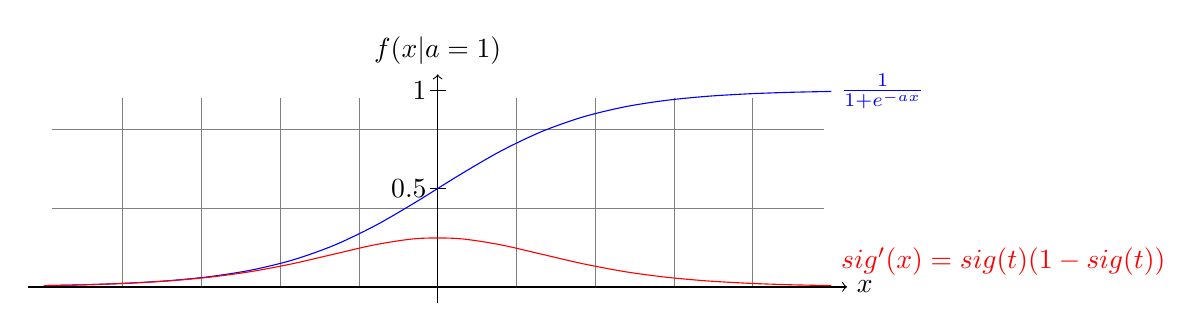
\begin{tikzpicture}[domain=-5:5, smooth, samples=20]
	\draw[very thin, color=gray] (-4.9,0.0) grid (4.9,2.4);

	\draw[->] (-5.2,0) -- (5.2,0) node[right] {$x$};
	\draw[->] (0,-0.2) -- (0,2.7) node[above] {$f(x|a=1)$};
	\draw (-0.1,2.5) --(0.1,2.5) node [left] {$1~$};
	\draw (-0.1,1.25) -- (0.1,1.25) node [left] {$0.5~$};

	\draw[color=blue] plot (\x,{2.5 / (1+exp(-\x))}) node[right] {$\frac{1}{1+e^{-ax}}$};
	\draw[color=red]  plot (\x,{2.5 / (1+exp(-\x)) * (1-1/(1+exp(-\x)))}) node[above right] {$sig'(x)=sig(t)(1-sig(t))$};
\end{tikzpicture}

